\documentclass[../differential_geometry.tex]{subfiles}
\begin{document}
\section{Aula 16 - 28 de Maio, 2026}
\subsection{Motivações}
\begin{itemize}
	\item A Derivada da Aplicação de Gauss;
	\item O Operador de Forma.
\end{itemize}
\subsection{O Operador de Forma}
Vimos que a derivada da aplicação de Gauss,
\[
	\mathrm{d}N_{p}:T_pS\rightarrow T_pS,
\]
é um oeprador auto-adjunto, significando algumas coisas:
\begin{itemize}
	\item[1)] Existe uma base ortonormal \(\{e_1, e_2\}\) em \(T_pS\) de autovetores de \(\mathrm{d}N_p\);
	\item[2)] \(\mathrm{d}N_p\) possui autovalores \(\lambda_1, \lambda_2\);
	\item[3)] O traço do operador, \(\mathrm{tr}(\mathrm{d}N_p)\), satisfaz
	      \[
		      \mathrm{tr}(\mathrm{d}N_p) = \lambda_1 \pm \lambda_2;
	      \]
	\item[4)] O determinante do operador satisfaz
	      \[
		      \mathrm{det}(\mathrm{d}N_p) = \lambda_1\lambda_2.
	      \]
\end{itemize}
O que seriam os significados geométricos, e como calcular, as propriedades de 1 a 4? Ora, começando por essa segunda, se \(\underline{x}:U\rightarrow \mathbb{R}^{3}\) for uma parametrização local, então \(\{\underline{x}_u, \underline{x}_v\}\) é uma base de \(T_pS\); logo, para \(v = T_pS\) e \(\underline{\ell }=\mathrm{d}N_p\), sabemos como calcular \(\lambda_{i}\) e \(f_{i}\)!

Para a pergunta, observe que \(\mathrm{d}N_p\) mede a variação do vetor normal à superfície, e portanto de seu plano tangente! Assim, é de se esperar que esta aplicação captura o jeito como S ``se curva'' no espaço \(\mathbb{R}^{3}\), determinando uma \textit{forma} assumida.

\begin{def*}
	O \textbf{operador de forma} ou \textbf{operador de Weingarten} de uma superfície S em \(\mathbb{R^{3}}\) no ponto p em S é o operador auto-adjunto
	\[
		W_p \coloneqq -\mathrm{d}N_p :T_pS\rightarrow T_pS.
	\]
	Os autovalores de \(W_p\) são chamadas \textbf{curvaturas principais}, denotadas por \(\kappa_1,\; \kappa_2\), de S no ponto p. \(\square\)
\end{def*}
As curvaturas principais satisfazem as soluções da equação
\[
	(EG-F^{2})\kappa^{2} - (\ell G - 2m F +nE)\kappa + \ell n - m^{2} = 0.
\]
\begin{def*}
	Os autovetores de \(W_p\) são as \textbf{direções principais} de S em p. \(\square\)
\end{def*}
Consequentemente, um vetor \(\alpha_1 \underline{x}_u + \alpha_2 \underline{x}_v\) é uma direção principal se, e somente se,
\[
	\det\begin{bmatrix}
		\alpha_{2}^{2} & -\alpha_1\alpha_2 & \alpha_{1}^{2} \\
		E              & F                 & G              \\
		\ell           & m                 & n
	\end{bmatrix} = 0.
\]
Caso \(\kappa_1\neq \kappa_2\), as direções principais são ortogonais. Além disso, podemos definir:
\begin{def*}
	A \textbf{curvatura gaussiana} \(\kappa \) de S em p é
	\[
		\kappa = \det{W_{p}} = \kappa_1 \kappa_2 = \frac{\ell n - m^{2}}{EG - F^{2}},
	\]
	a \textbf{curvatura média} H de S em p é
	\[
		H = \frac{1}{2}\mathrm{tr}(W_p) = \frac{1}{2}(\kappa_1+\kappa_2)=\frac{\ell G - 2mF +nE}{2(EG-F^{2})},
	\]
	e um ponto p em S é um \textbf{ponto umbilical} se \(\kappa_1 = \kappa_2.\; \square\)
\end{def*}
Como encontrar \(\ell ,\; m\) e n? Bom, temos as seguintes relações:
\begin{align*}
	 & \ell =\langle W_p(\underline{x}_u), \underline{x}_u  \rangle                                                      \\
	 & m = \langle W_p(\underline{x}_u), \underline{x}_v \rangle = \langle \underline{x}_u, W_p(\underline{x}_v) \rangle \\
	 & n = \langle W_p(\underline{x}_v), \underline{x}_v \rangle.
\end{align*}
Com a notação \(N_u = \mathrm{d}N_p(\underline{x}_u) = - W_p(\underline{x}_u)\), e como \(\langle N, \underline{x}_u \rangle = 0\) (afinal, N é normal a \(\underline{x}_u\)), temos:
\[
	\langle N_u, \underline{x}_u \rangle + \langle N, \underline{x}_{uu} \rangle = 0.
\]
Logo,
\[
	\langle -N_u, \underline{x}_u \rangle = \langle N, \underline{x}_{uu} \rangle,
\]
e, portanto,
\[
	\boxed{\ell = \langle N, \underline{x}_{uu} \rangle}, \quad  \boxed{m = \langle N, \underline{x}_{uv} \rangle} \quad\&\quad \boxed{n = \langle N, \underline{x}_{vv} \rangle}
\]
\begin{example}
	Seja S o gráfico da função \(z = \frac{x^{2}-y^{2}}{2}\); uma parametrização local de S é
	\[
		\underline{x}(u, v) = \biggl(u, v, \frac{1}{2}(u^{2}-v^{2})\biggr), \quad (u, v)\in \mathbb{R}^{2},
	\]
	donde obtemos
	\[
		\underline{x}_u = (1, 0, u) \quad\&\quad \underline{x}_v = (0, 1, v),
	\]
	de modo que
	\[
		\underline{x}_{uu} = (0, 0, 1), \quad \underline{x}_{uv} = (0, 0, 0) \quad\&\quad \underline{x}_{vv} = (0, 0, -1).
	\]
	Portanto,
	\[
		N(u, v) = \frac{\underline{x}_u(u, v)\times \underline{x}_v(u, v)}{\Vert \underline{x}_u(u, v)\times \underline{x}_v(u, v) \Vert} = \frac{(-u, v, 1)}{\sqrt[]{1+u^{2}+v^{2}}}.
	\]
	Para o próximo raciocínio, vamos denotar a por \(\Delta \) o termo \(\Delta \coloneqq 1+u^{2}+v^{2}\).

	Com isso, obtemos os coeficientes da primeira forma fundamental como sendo
	\begin{align*}
		 & E = \langle \underline{x}_u, \underline{x}_u \rangle  = 1+u^{2}  \\
		 & F = \langle \underline{x}_u, \underline{x}_v \rangle  = -uv      \\
		 & G = \langle \underline{x}_v, \underline{x}_v \rangle  = 1+v^{2},
	\end{align*}
	e, em particular,
	\[
		EG - F^{2} = 1 + u^{2} + v^{2} + u^{2}v^{2}-u^{2}v^{2} = \Delta.
	\]
	Daí, os coeficientes \(\ell ,\; n\) e \(m\) são dados por:
	\begin{align*}
		 & \langle N, \underline{x}_{uu} \rangle = \frac{1}{\sqrt[]{\Delta }}\langle (-u, v, 1),(0, 0, 1)  \rangle = \frac{1}{\sqrt[]{\Delta }} \\
		 & m = \langle N, \underline{x}_{uv} \rangle = 0                                                                                        \\
		 & n = \langle N, \underline{x}_{vv} \rangle = - \frac{1}{\sqrt[]{\Delta }},
	\end{align*}
	tal que
	\[
		\ell n - m^{2} = - \frac{1}{\Delta }.
	\]

	Além disso, conseguimos as curvaturas gaussiana e média com
	\begin{align*}
		 & \kappa  = \frac{\ell n-m^{2}}{EG-F^2} = -\frac{1}{\Delta^{2}}                                                                                      \\
		 & H = \frac{1}{2}\mathrm{tr}(W_{p}) = \frac{1}{2}\frac{\ell G - 2mF + nE}{EG-F^{2}}                                                                  \\
		 & \quad = \frac{1}{2}\frac{\frac{1+u^{2}}{\sqrt[]{\Delta }}- \frac{1+v^{2}}{\sqrt[]{\Delta }}}{\Delta } = \frac{v^{2}-u^{2}}{2\Delta^{\frac{3}{2}}}.
	\end{align*}
	Logo, as curvaturas principais serão dadas pela soluções de
	\[
		\kappa ^{2} - 2H\kappa  + K  =0 \Longleftrightarrow \kappa ^{2} - \frac{v^{2}u-u^{2}}{\Delta^{\frac{3}{2}}}\kappa -\frac{1}{\Delta^{2}}=0,
	\]
	resultando em
	\[
		\delta = \frac{(v^{2}-u^{2})^{2}\Delta +4}{\Delta^{4}}
	\]
	e nas soluções
	\[
		\kappa_{i} = \frac{1}{2}\biggl(\frac{v^{2}-u^{2}}{\Delta^{\frac{3}{2}}} + (-1)^{i}\frac{1}{\Delta^{2}}\sqrt[]{(v^{2}-u^{2})^{2}\Delta +4}\biggr), \quad i=1, 2.
	\]

	Finalmente, as direções principais serão os vetores que resolvem
	\[
		\det\begin{bmatrix}
			\alpha_{2}^{2}             & -\alpha_1\alpha_2 & \alpha_{1}^{2}               \\
			1+u^{2}                    & -uv               & 1+v^{2}                      \\
			\frac{1}{\sqrt[]{\Delta }} & 0                 & - \frac{1}{\sqrt[]{\Delta }}
		\end{bmatrix} = 0 \Longleftrightarrow uv \alpha_{2}^{2} - (2+u^{2}+v^{2})\alpha_1\alpha_2 + uv\alpha_{1}^{2} = 0.
	\]
\end{example}
\subsection{A Segunda Forma Fundamental}
Seja S uma superfície em \(\mathbb{R}^{3}\).
\begin{def*}
	A \textbf{segunda forma fundamental} de S no ponto p é a aplicação bilinear e simétrica
	\[
		\mathbb{I}_p:T_pS\times T_pS\rightarrow \mathbb{R}
	\]
	dada por
	\[
		\mathbb{I}_p (w_1, w_2) = \langle W_p(w_1), w_2 \rangle = \langle w_1, W_p(w_2) \rangle.\; \square
	\]
\end{def*}

À forma quadrática \(\mathbb{I}_{p}\), associamos
\[
	\mathbb{I}_{p}(w) = \mathbb{I}_{p}(w, w) = \langle W_p(w), w \rangle, \quad w\in T_pS.
\]
Disso, se \(\underline{x}:U\rightarrow \mathbb{R}^{3}\) é uma parametrização local de S e \(p=\underline{x}(u, v)\), para \(w = a \underline{x}_u + b\underline{x}_v\) em \(T_pS\), teremos
\begin{align*}
	\mathbb{I}_p(w) & = \langle W_p(a\underline{x}_u + b\underline{x}_v), a\underline{x}_u + b\underline{x}_v \rangle          \\
	                & = \langle a W_p(\underline{x}_u) + b W_p(\underline{x}_v), a \underline{x}_u + b \underline{x}_v \rangle \\
	                & = a^{2}\ell +2ab m + b^{2}n.
\end{align*}
\begin{def*}
	Os coeficientes \(\ell , m\) e n são chamados \textbf{coeficientes da segunda forma fundamental}. \(\square\)
\end{def*}
\begin{example}[Segunda Forma Fundamental do Gráfico de Função Suave]
	O gráfico de uma função suave \(g:U\subseteq \mathbb{R}^{2}\rightarrow \mathbb{R}\) tem uma parametrização usual dada por
	\[
		\underline{x}(u, v) = (u, v, g(u, v)).
	\]
	Assim, temos:
	\begin{align*}
		 & \underline{x}_u = (1, 0, g_u)        \\
		 & \underline{x}_v = (0, 1, g_v)        \\
		 & \underline{x}_{uu} = (0, 0, g_{uu})  \\
		 & \underline{x}_{uv} = (0, 0, g_{uv})  \\
		 & \underline{x}_{uu} = (0, 0, g_{vv}).
	\end{align*}
	Logo,
	\[
		\begin{bmatrix}
			\hat{i} & \hat{j} & \hat{k} \\
			1       & 0       & g_u     \\
			0       & 1       & g_v
		\end{bmatrix} = (-g_u, -g_v, 1)
	\]
	e
	\[
		N = \frac{(-g_u, -g_v, 1)}{\sqrt[]{1 + g_{u}^{2} + g_{v}^{2}}}.
	\]
	Concluímos, então, que os coeficientes da segunda forma fundamental do gráfico de uma função suave são dados por:
	\begin{align*}
		 & \ell  = \langle N, \underline{x}_{uu} \rangle = \frac{g_{uu}}{\sqrt[]{1+g_u^{2}+g_{v}^{2}}} \\
		 & m = \langle N, \underline{x}_{uv} \rangle = \frac{g_{uv}}{\sqrt[]{1+g_u^{2}+g_{v}^{2}}}     \\
		 & n = \langle N, \underline{x}_{vv} \rangle = \frac{g_{uv}}{\sqrt[]{1+g_u^{2}+g_{v}^{2}}}.
	\end{align*}
\end{example}

No entanto, temos um pequeno problema, e ele é relacionado à interpretação geométrica da segunda forma fundamental, afinal ela não é tão direta quanto a primeira. Para tanto, temos que introduzir alguns conceitos, especificamente o conceito de \textit{curvatura geodésica} e o de \textit{curvatura normal}.

Seja \(\beta \) uma curva regular em S, parametriza por comprimento de arco; considerando \(\beta \) como uma curva em \(\mathbb{R}^{3}\), temos:
\[
	\frac{\mathrm{d}\beta }{\mathrm{d}s} =\beta'= t \quad\&\quad \frac{\mathrm{d}^{2}\beta }{\mathrm{d}s^{2}} = \beta''=t'=\kappa n,
\]
onde \(\kappa \) é a curvatura de \(\beta \) como curva em \(\mathbb{R}^{3}\).

Como \(\beta \) é unitário,
\[
	\langle \beta ', \beta ' \rangle = 1 \Rightarrow \langle \beta '', \beta '' \rangle = 0,
\]
e, consequentemente, \(\beta ''\) pertence ao plano gerado por N e \(N\times t\), onde N é o vetor normal à superfície S no ponto \(\beta (s)\).
Deste modo, existem escalars \(\kappa_{g}(s)\) e \(\kappa_{n}(s)\) tais que
\[
	\beta''= \kappa_{g}N\times t + \kappa_{n} N.
\]
O primeiro, \(\kappa_{g}\), representa a componente tangencial equivalente à aceleração; o segundo, por sua vez, representa a componente normal da aceleração! Por isso, recebem os nomes:
\begin{def*}
	O coeficiente \(\kappa_{n}\) é a \textbf{curvatura normal de \(\mathbf{\beta }\)}, e \(\kappa_{g}(s)\) é a \textbf{curvatura geodésica de \(\mathbf{\beta }\)}. \(\square\)
\end{def*}
\begin{figure}[H]
	\begin{center}
		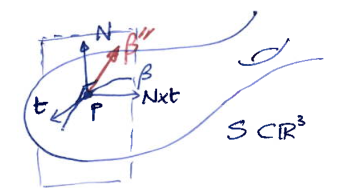
\includegraphics[height=0.5\textheight, width=0.5\textwidth, keepaspectratio]{./Images/normal_curvature_17.png}
	\end{center}
\end{figure}
Considerando \(\beta \) como uma curva em \(\mathbb{R}^{3}\), temos \(\beta ''= \kappa n\), tal que
\[
	\kappa n = \kappa_{g} N\times t + \kappa_{n}N,
\]
e por \(n, N\times t\) e N serem todo unitários, além de \(\langle N\times t, N \rangle = 0\), obtemos
\[
	\boxed{\kappa^{2} = \kappa_{g}^{2} + \kappa_{n}^{2}}
\]
Vamos supor, agora, que \(\beta \) é a curva obtida pela interseção da superfície S com um plano passando por p em S e gerado por \(N(p)\), e que \(w\in T_pS\) com w unitário. Neste caso, \(\beta''\) é paralelo a N, e portanto
\[
	\kappa_{g} = 0 \Rightarrow \kappa = \pm \kappa_{n}.
\]
\begin{figure}[H]
	\begin{center}
		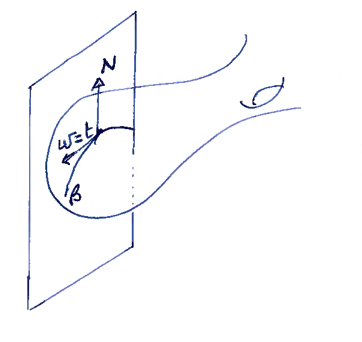
\includegraphics[height=0.7\textheight, width=0.7\textwidth, keepaspectratio]{./Images/observation_17.png}
	\end{center}
\end{figure}
\end{document}
